%%%%%%%%%%%%%%%%%%%%%%%%%%%%%%%%%%%%%%%%%
% University/School Laboratory Report
% LaTeX Template
% Version 3.1 (25/3/14)
%
% This template has been downloaded from:
% http://www.LaTeXTemplates.com
%
% Original author:
% Linux and Unix Users Group at Virginia Tech Wiki 
% (https://vtluug.org/wiki/Example_LaTeX_chem_lab_report)
%
% License:
% CC BY-NC-SA 3.0 (http://creativecommons.org/licenses/by-nc-sa/3.0/)
%
%%%%%%%%%%%%%%%%%%%%%%%%%%%%%%%%%%%%%%%%%

%----------------------------------------------------------------------------------------
%	PACKAGES AND DOCUMENT CONFIGURATIONS
%----------------------------------------------------------------------------------------

\documentclass[11pt]{article}

% \usepackage[version=3]{mhchem} % Package for chemical equation typesetting
% \usepackage{siunitx} % Provides the \SI{}{} and \si{} command for typesetting SI units
\usepackage{graphicx} % Required for the inclusion of images
\usepackage[center]{caption}
\usepackage{subcaption}
\usepackage{algorithm}
\usepackage{algpseudocode}
% \usepackage{natbib} % Required to change bibliography style to APA
\usepackage{amsmath} % Required for some math elements 
\usepackage{amssymb}
\usepackage{setspace}
\usepackage{geometry}
\usepackage{helvet}
\usepackage{wrapfig}
% \renewcommand{\familydefault}{\sfdefault}
\geometry{margin=20mm}
\setlength\parindent{0pt} % Removes all indentation from paragraphs
\setstretch{2}
\renewcommand{\labelenumi}{\alph{enumi}.} % Make numbering in the enumerate environment by letter rather than number (e.g. section 6)
\setlength{\parskip}{-1em}
\newcommand{\icol}[1]{% inline column vector
  \left(\begin{smallmatrix}#1\end{smallmatrix}\right)%
}

%\usepackage{times} % Uncomment to use the Times New Roman font

%----------------------------------------------------------------------------------------
%	DOCUMENT INFORMATION
%----------------------------------------------------------------------------------------

\title{B1 Computational Project Report \\ Neural Network Verification} % Title

\author{Candidate Number: 1044559} % Author name

\date{Michaelmas 2021} % Date for the report

\begin{document}

\maketitle % Insert the title, author and date

% \begin{center}
% \begin{tabular}{l r}
% Date Performed: & December 13, 2021 \\ % Date the experiment was performed
% Instructor: & Professor Smith % Instructor/supervisor
% \end{tabular}
% \end{center}

% If you wish to include an abstract, uncomment the lines below
% \begin{abstract}
% Abstract text
% \end{abstract}

%----------------------------------------------------------------------------------------
%	SECTION 1
%----------------------------------------------------------------------------------------

\section{Introduction}
Throughout this document we will refer to the Neural Networks (NN) from the collision detection dataset~\cite{DBLP:journals/corr/Ehlers17} from which the weights and biases have been provided as \textbf{examples}.
We will \textbf{classify} examples as $1$ (true) if it is proven that there is no possible output from the network that is positive, and $0$ (false) if it is proven that there exists at least one positive output.
The function \texttt{get\_ground\_truth} was written to help verify results given by the tasks. 
The function uses the \texttt{groundtruth.txt} file given and converts this into a $500\times1$ vector in which a $1$ and $0$ are have the same meanings as above.
We will say an output has been \textbf{correctly classified} or \textbf{verified} if the classification of a given example is the same as the ground truth.
We will define $y^*$ as the maximum possible output from the network given the bounded inputs.
The computations for each example are independent of one another and thus are prime candidates for parralleisation.
We used the \texttt{parfor} loop from the \texttt{matlab} parralleisation toolbox to quarter computation time.
We were able to test four examples at once since the computer we used had four cores.
\section{Tasks}

%----------------------------------------------------------------------------------------
%	TASK 1
%----------------------------------------------------------------------------------------

\subsection{Task 1 - Random Sampling}
\subsubsection{Method}
% This problem is broken down into two functions with a script to combine them. 
% The first function, \texttt{generate\_inputs}, gernerates  $k$ random vectors $\boldsymbol{x}$ with elementwise values between the vectors $\boldsymbol{x}_{min}$ and $\boldsymbol{x}_{max}$. 
% The second function, \texttt{compute\_nn\_outputs}, conducts a forward pass through the neural network to obtain samples of possible outputs in the range of inputs.
\paragraph{Function \texttt{generate\_inputs}}
% We utilise the \texttt{rand} function with dimensions \texttt{(6,k)}, 6 representing the number of neurons in the first layer of the network and $k$ representing the number of inputs to be generated.
% We conduct an elementwise multiplication of this matrix by the column vector ${\boldsymbol{x}^T_{max}} - {\boldsymbol{x}^T_{min}}$ and add ${\boldsymbol{x}^T_{min}}$. 
% This spreads out the values of the matrix and shifts them such that each element is disributed uniformly in the ranges $[\boldsymbol{x}^T_{min},\boldsymbol{x}^T_{max}]$. 
This function is expressed as follows:
\begin{verbatim}
    X = (xmax-xmin)'.*rand(6,k) + xmin';
\end{verbatim}
\paragraph{Function \texttt{compute\_nn\_outputs}}
This function works much like \textbf{Algorithm 1} from~\cite{NNVNotes} however, we utilise a for loop iterating through the integers $1,2,\dots,L-1$ rather than a while loop.
\paragraph{Script}
The script for Task 1 is described by \textbf{Algorithm \ref{alg:Task1}}.
It is notable that the $\boldsymbol{y}$ vector is initialised containing $-\infty$. This is done as we are using the maximum function to update it and thus, if it were intialised as zeros, negative lower bounds would never be registered.
% We being this task by initialising our $t$ matrix and $y$ vector, representing time taken to generate the outputs of the neural network for every combination of example and $k_{max}$, as well as the maximum lower bound for the neural network respectively.
% $t$ is intilised using the \texttt{zeros} function and $y$ is initilaised using the \texttt{ones} function multiplied by $-\infty$
% We then iterate across all 500 examples and for each example load in the corresponding weights, biases, $x_{min}$ and $x_{max}$ using the \texttt{load} function as well as for every value of $k$: 1,2,\dots,$k_{max}$ generating $k$ inputs and recording the maximum lower bound for $y^*$ seen so far by finding a maximum across all $k$ inputs and comparing to the maximum seen before for this example.
% We time this process using the \texttt{tic} and \texttt{toc} functions and record these times to the $t$ matrix.
% Finally we plot two graphs, one of the mean time to generate the outputs from the neural network agains the value of k and another of the maximum lower bound for each example.
% We also calculate the number of properties for which a counter example by checking elementwise whether $y>0$ and summing up the resulting vector of booleans. 
\begin{algorithm}
    \caption{Task 1 script}\label{alg:Task1}
    \begin{algorithmic}
    \State Initialise $\boldsymbol{T}$ \Comment{Representing time. Initialised as a matrix of zeros}
    \State Initialise $\boldsymbol{y}$ \Comment{Representing the lower bound on $y^*$. Initialised as a vector of $-\infty$}
    \For {each example}
    \State load in weights and biases
    \For {$k \in 1,2,\dots,k_{max}$}
    \State $\boldsymbol{X} \gets$ generate inputs
    \State compute nn outputs
    \State update $\boldsymbol{y}$ with maximum $y$ across all $k$ and previous maximum for this example
    \EndFor
    \EndFor
    % \State plot mean time for generation against value of $k$
    % \State plot lower bound on $y_{max}$ against example number
    % \State calculate number of examples for which the lower bound on $y_{max}>0$ \Comment{And thus the number of examples we can classify as false} 
    \end{algorithmic}
\end{algorithm}
\subsubsection{Results}
The plots from Task 1 are shown in figure \ref{fig:Task1a} and figure \ref{fig:Task1b}. 
Figure \ref{fig:Task1a} shows the mean time taken linearly increasing with $k$. 
There is a signifcant amount of noise present even when there is no other applications running in the foreground.
% Figure \ref{fig:Task1b} shows a noisy increase in lower bound with example number which flattens at 150. There is no reason to expect a trend in this data as examples are assumed to be uncorrelated. 
% However, this general shape does continue for time plotted against example number throughout the tasks leading to the conclusion that in general, later examples are more difficult. \\
We obtained a mean lower bound on $y^*$ of $-19.2$ and with $k_{max}=1000$ were able to correctly classify 125 out of a total of 172 possible examples as false.
\begin{figure}
    \centering
    \begin{subfigure}{.5\textwidth} 
        \centering 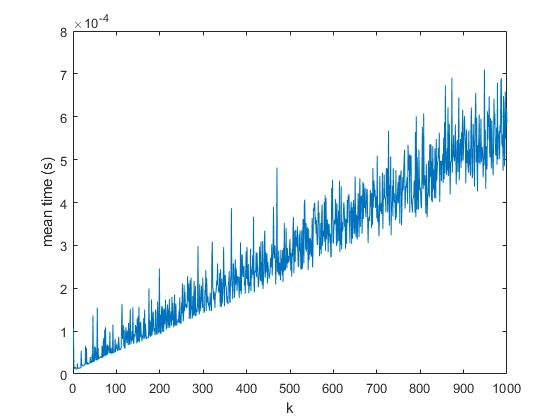
\includegraphics[width=0.8\columnwidth]{Figures/Task1tvk.jpg}
        \caption{\label{fig:Task1a}$k$ against the mean time in seconds for the calculation of the neural network outputs across all examples. With $k_{max}=1000$
        }
    \end{subfigure}%
    \begin{subfigure}{.5\textwidth} 
        \centering 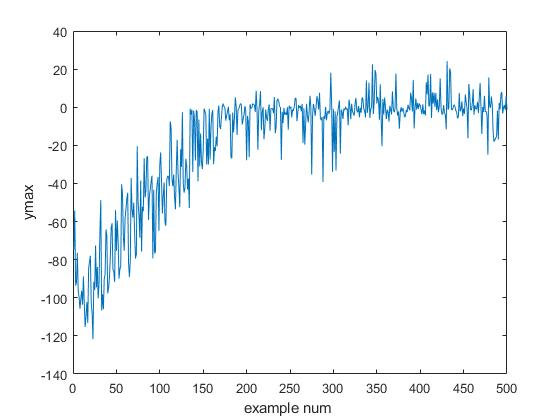
\includegraphics[width=0.8\columnwidth]{Figures/Task1yvexample.jpg}
        \caption{\label{fig:Task1b}The value of the lower bound on $y^*$ against the example number.
        }
    \end{subfigure}
    \caption{}
    \label{fig:Task1}
\end{figure}
\subsubsection{Discussion}
This method is very fast, taking less that $10^{-3}$s with $k=1000$, and produces a good quality lower bound on $y^*$. 
These small times are responsible for the noise in figure \ref{fig:Task1a}, as the time taken for background processes on the machine becomes significant.
Due to its random nature, it is not guaranteed to generate a good quality bound on $y^*$, and in turn a counter example for an example classified as false. 
It is not capable of classifying an example as true.
Although this method alone is incomplete for calssifying examples, it is very useful during the \texttt{branch\_and\_bound} procedure in Task 3. 
Unlike other methods which find a lower bound on $y$, it finds a lower bound on $y^*$.
This helps to raise the lower bound faster and speed up convergence. 
It is notable that the bounds on $y^*$ as opposed to $y$ allow us to classify the example and thus are the bounds we are more interested in.

%----------------------------------------------------------------------------------------
%	TASK 2
%----------------------------------------------------------------------------------------

\subsection{Task 2 - Interval Bound Propogation}

\subsubsection{Method}

% This problem is broken down into the function \texttt{interval\_bound\_propogation} and a script to evaluate it.

\paragraph{Function \texttt{interval\_bound\_propogation}} This function is best described by \textbf{Algorithm \ref{alg:IntBounProp}}.
\begin{algorithm}
    \caption{Interval Bound Propogation}\label{alg:IntBounProp}
    \begin{algorithmic}
        \State Initialise $\boldsymbol{z}_{min}$ as $\boldsymbol{x}_{min}^T$
        \State Initialise $\boldsymbol{z}_{max}$ as $\boldsymbol{x}_{max}^T$
        \For {$l \in 1,2,\dots,L-1$} \Comment{The last layer does not have a ReLU}
            \State $\boldsymbol{W}^- \gets min(0,\boldsymbol{W}_l)$ \Comment{$min$ operates elementwise}
            \State $\boldsymbol{W}^+ \gets max(0,\boldsymbol{W}_l)$ \Comment{$max$ operates elementwise}
            \State $\boldsymbol{z}_{min}^{temp} \gets \boldsymbol{z}_{min}$
            \State $\boldsymbol{z}_{min} \gets max(0,\boldsymbol{W}^+\boldsymbol{z}_{min}+\boldsymbol{W}^-\boldsymbol{z}_{max} + \boldsymbol{b}_l)$
            \State $\boldsymbol{z}_{max} \gets max(0,\boldsymbol{W}^+\boldsymbol{z}_{max}+\boldsymbol{W}^-\boldsymbol{z}_{min} + \boldsymbol{b}_l)$
        \EndFor
        \State $\boldsymbol{W}^- \gets min(0,\boldsymbol{W}_L)$
        \State $\boldsymbol{W}^+ \gets max(0,\boldsymbol{W}_L)$
        \State $\boldsymbol{z}_{min}^{temp} \gets \boldsymbol{z}_{min}$
        \State $z_{min} \gets \boldsymbol{W}^+\boldsymbol{z}_{min}+\boldsymbol{W}^-\boldsymbol{z}_{max} + \boldsymbol{b}_L$
        \State $z_{max} \gets \boldsymbol{W}^+\boldsymbol{z}_{max}+\boldsymbol{W}^-\boldsymbol{z}_{min} + \boldsymbol{b}_L$ 
        \State $y_{min} \gets z_{min}$
        \State $y_{max} \gets z_{max}$
    \end{algorithmic}
\end{algorithm}

\paragraph{Script} The script for Task 2 is described by \textbf{Algorithm \ref{alg:Task2}}. 
It is notable that $\boldsymbol{Y}$ is initilaised as a $2\times500$ matrix as each column is the vector 
$\big[\begin{smallmatrix} 
    y_{min} \\ 
    y_{max} 
\end{smallmatrix}\big]$.

\begin{algorithm}
    \caption{Task 2 script}\label{alg:Task2}
    \begin{algorithmic}
    \State Initialise $\boldsymbol{Y}$ \Comment{Initialised as a $2\times500$ matrix of zeros}
    \For {each example}
    \State load in weights and biases
        \State interval bound propogation
        \State update $\boldsymbol{Y}$ matrix with $y_{min}$ and $y_{max}$
    \EndFor
    % \State plot $y_{min}$ and $y_{max}$ against example number
    % \State calculate number of examples for which $y_{min}>0$ \Comment{And thus the number of examples we can classify as false} 
    % \State calculate number of examples for which $y_{max}<0$ \Comment{And thus the number of examples we can classify as true} 
\end{algorithmic}
\end{algorithm}

\subsubsection{Results}
\begin{figure}
    \begin{subfigure}{.5\textwidth}%
        \centering 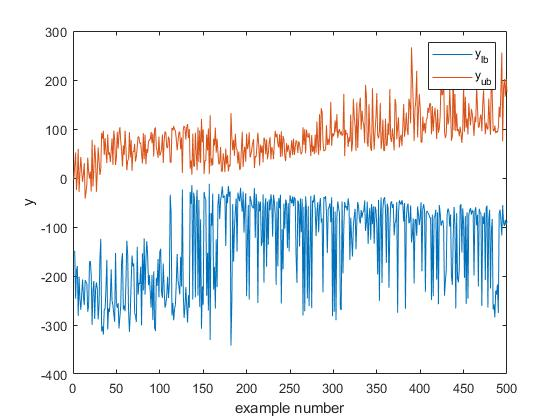
\includegraphics[width=0.8\columnwidth]{Figures/task2.jpg}
        \caption{The upper and lower bounds on $y$ as obtained by \texttt{interval\_bound\_propogation} in Task 2 against example number}
        \label{fig:Task2}
    \end{subfigure}
    \begin{subfigure}{.5\textwidth} 
        \centering 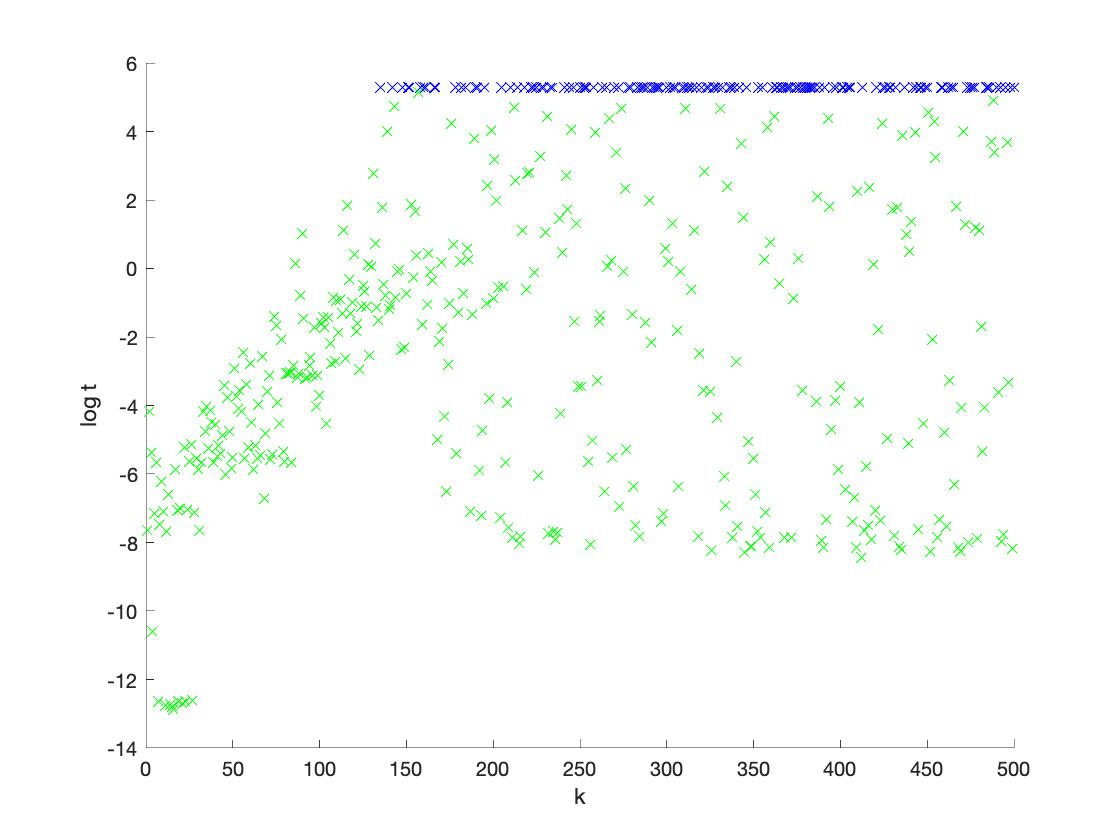
\includegraphics[width=0.8\columnwidth]{Figures/Task3.jpg}
        \caption{The log of the time taken for the \texttt{branch\_and\_bound} procedure to converge in Task 3 against the example number. Examples classified correctly are shown in green and examples which did not converge are shown in blue.}
        \label{fig:Task3}
    \end{subfigure}
    \caption{}
\end{figure}

The plot for Task 2 is show in figure \ref{fig:Task2}. 
We obtained a mean lower bound on $y$ of -137.9 and a mean upper bound on $y$ of 82.7. 
We were also able to correctly classify 0 examples as false and 11 examples as true. 
\subsubsection{Discussion}
The \texttt{interval\_bound\_propogation} method produces valid bounds, however, they are very loose as shown by the small number of examples for which we obtained a classification and the poor lower bound in comparison to the \texttt{random\_sampling} in Task 1.
This is becuase the bounds produced are on $y$ rather than $y^*$ 
i.e. the lower bound is a bound on the lowest possible output of the neural network. The upper bound of $y$ is the same as that of $y^*$.
% It is also notable that interval bound propogation produces a lower bound on $y$ rather than a lower bound on $y_{max}$. This results in a much looser, and thus less useful, lower bound than the random sampling from Task 1.

%----------------------------------------------------------------------------------------
%	TASK 3
%----------------------------------------------------------------------------------------

\subsection{Task 3 - Branch and Bound}
\subsubsection{Method}
\paragraph{Function \texttt{random\_sampling}}
This works the same as Task 1, however, it has been reformulated into a function outputting the maximum output generated.
\paragraph{Function \texttt{branch\_and\_bound}}
This function works much like \textbf{Algorithm 1} from~\cite{NEURIPS2018_be53d253} however, because our criteria for example classification are opposite, we maximise the lower bound rather than minimise the upper bound. 
We use \texttt{interval\_bound\_propogation} to generate the upper bounds and the maxmimum lower bound from \texttt{random\_sampling}, and \texttt{interval\_bound\_propogation} as our lower bound. 
It is possible that the lower bound generated is greater than the upper bound.
When this occurs we take the upper bound of the subdomain to be the same as the lower bound.
In place of the \texttt{pick\_out} function we choose the domain with the maximum upper bound. This domain is removed from the set and split into subdomains. 
In place of the \texttt{split} function we cut along the longest edge as stated in~\cite{NNVNotes}.
% In order to prune domains we remove domains where the upper bound is less than the global lower bound as these are not useful for obtaining a classification. 
As we are only looking for a classification we followed the recommendation of~\cite{NEURIPS2018_be53d253} and set the global lower bound to zero. 
It is thus uncessary to prune domains as any situation in which this would be necessary would be a counter example and so we return a false classification.
Due to some examples taking a very long time to run we set a limit for each example. If the result did not converge within this time we set the flag to $-1$ to indicate there is no classification.
\paragraph{Script}
In order to evaluate \texttt{branch\_and\_bound} we first initialise our $\boldsymbol{y}_{flags}$ and $\boldsymbol{t}$ vectors. 
Then for each example we:
load in the weights and biases;
run the \texttt{branch\_and\_bound} procedure while recording the time it takes;
record the output into the $\boldsymbol{y}_{flags}$ vector and the time taken into the $\boldsymbol{t}$ vector;
and finally we verify our outputs and plot the graph.
\subsubsection{Results} The plot for Task 3 is shown in figure \ref{fig:Task3}.
Out of the 500 examples 367 converged and we were able to verify all of these outputs. 
We used a time limit of 200 seconds for each example, $\epsilon=0.1$ and $k=300$ for \texttt{random\_sampling}. 
The script was left running overnight and took around 8 hours to complete.
 
% \begin{figure}
%     \centering
%         \centering 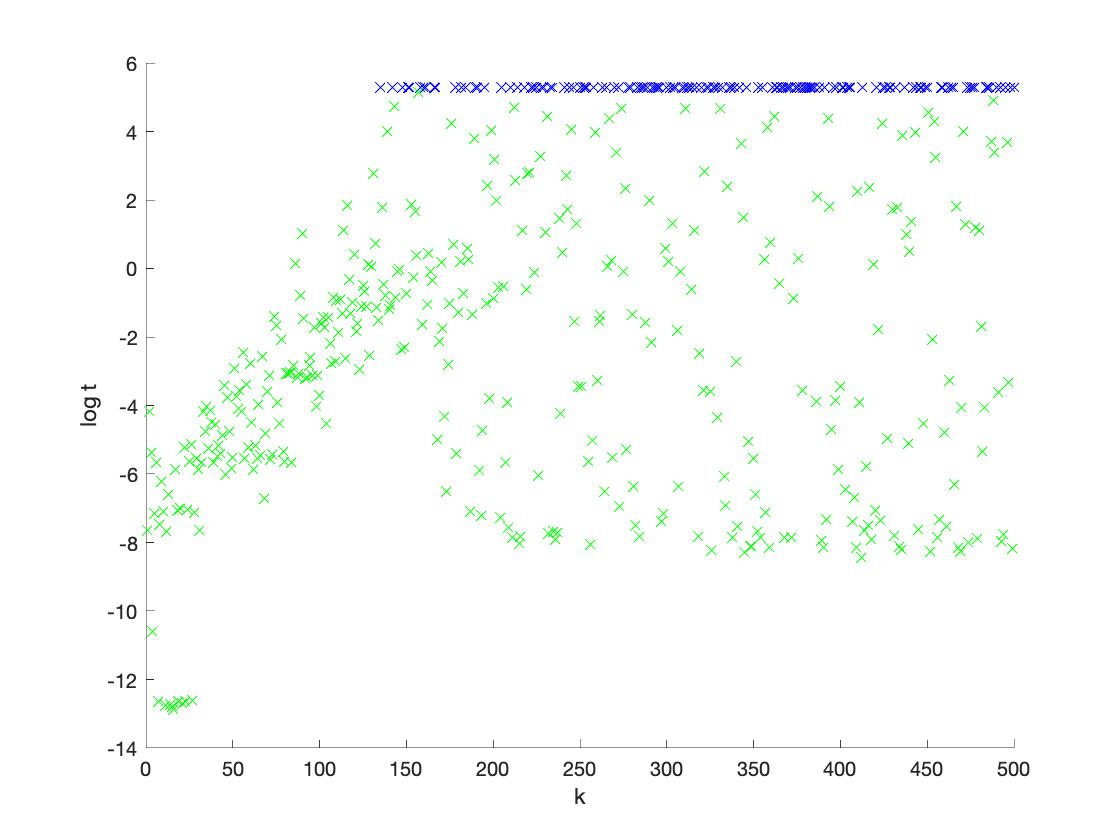
\includegraphics[width=0.4\columnwidth]{Figures/Task3.jpg}
%     \caption{The log of the time taken for the branch and bound procedure to converge in Task 3 against the example number. Examples classified correctly are shown in green and examples which did not converge are shown in blue.}
%     \label{fig:Task3}
% \end{figure}

\subsubsection{Discussion}
The \texttt{branch\_and\_bound} procedure provides a very flexible and powerful method for classifying examples. 
The main constraint on the rate of convergence is the quality of the bounds on $y^*$ calculated for each subdomain.
When the bounds have converged we have classified the examples as tentatively true, as it is likely the upper bound will continue to decrease below zero. 
However, it is possible that $0<y^*<\epsilon$.
In this case our tentative classification would be incorrect. 
The probability of this occuring decreases with $\epsilon$ but the computation time increases.
We chose our value of $\epsilon$ as it is small enough to allow correct classification of most examples, but not to prohibitively increase computation time. 
We chose our value of $k$ to balance the quality of the bounds generated and the computation time.

%----------------------------------------------------------------------------------------
%	TASK 4
%----------------------------------------------------------------------------------------

\subsection{Task 4 - Projected Gradient Descent}
\subsubsection{Method}
\paragraph{Function \texttt{projected\_gradient\_ascent}}
% This function is descirbed by algorithm \ref{alg:Task4}
This function takes the $n\times m$ matrix $\boldsymbol{X}$ and for each column $\boldsymbol{x}$ calculates an updated version $\boldsymbol{x}^{new}$. 
The calculation of the gradient wrt $\boldsymbol{x}$ for this neural network is shown in \textbf{Equation \ref{eq:Task4}}.
We iterate through the neural network where in each layer we calculate a value of $\boldsymbol{z}$ and track the gradient at this layer i.e. calculate $\frac{\partial \boldsymbol{z}_l}{\partial \boldsymbol{x}}$. 
We then update $\boldsymbol{x}$ with the calculated gradient at a given learning rate $\eta$. 
Finally we take take $x^{new}_i = min(x^{new}_i,x^{max}_i)$ and $x^{new}_i = max(x^{new}_i,x^{min}_i)$ to keep $\boldsymbol{x}^{new}$ within the domain.
We repeat this for $n$ iterations for every $\boldsymbol{x} \in columns(\boldsymbol{X})$.
\begin{align}
	\frac{\partial y}{\partial \boldsymbol{x}} &= \frac{\partial y}{\partial \boldsymbol{z}_4}\frac{\partial \boldsymbol{z}_4}{\partial \hat{\boldsymbol{z}}_4}\frac{\partial \hat{\boldsymbol{z}}_4}{\partial \boldsymbol{z}_3}\frac{\partial \boldsymbol{z}_3}{\partial \hat{\boldsymbol{z}}_3}\frac{\partial \hat{\boldsymbol{z}}_3}{\partial \boldsymbol{z}_2}\frac{\partial \boldsymbol{z}_2}{\partial \hat{\boldsymbol{z}}_2}\frac{\partial \hat{\boldsymbol{z}}_2}{\partial \boldsymbol{z}_1}\frac{\partial \boldsymbol{z}_1}{\partial \hat{\boldsymbol{z}}_1}\frac{\partial \hat{\boldsymbol{z}}_1}{\partial \boldsymbol{x}} 
    &     
    \text{where } \boldsymbol{x}& \in \mathbb{R}^n \text{ and the } n\times n \text{ matrix}, \notag 
    \\
	&=\boldsymbol{W}_5 R^\prime (\hat{\boldsymbol{z}}_4) \boldsymbol{W}_4 R^\prime (\hat{\boldsymbol{z}}_3) \boldsymbol{W}_3 R^\prime (\hat{\boldsymbol{z}}_2) \boldsymbol{W}_2 R^\prime (\hat{\boldsymbol{z}}_1) \boldsymbol{W}_1  
    & 
    R^\prime(\boldsymbol{x})& = 
    \begin{cases}
        0,& \text{if } i \neq j\\
        0,              & \text{if } x_{i,j} \leq 0  \text{ and } i=j\\
        1, & \text{if } x_{i,j} > 0  \text{ and } i=j
    \end{cases} \notag
    \\
    &= \boldsymbol{W}_5 \prod_{k=4,3,2,1} R^\prime (\hat{\boldsymbol{z}}_k) \boldsymbol{W}_k  \label{eq:Task4}
    % \text{where} \; R(\boldsymbol{x}) = max(0,\boldsymbol{x}) \; \text{elementwise}\notag\\
    % \text{and} \; R^\prime(\boldsymbol{x}) = \frac{\partial R^\prime(\boldsymbol{x})}{\partial \boldsymbol{x}} = 
    % \begin{bmatrix}
    %     max(0,x_{1,1}>0) & 0 & \dots & 0 \\
    %     0 & max(0,x_{2,2}>0) & \dots & 0 \\
    %     \vdots & \vdots & \ddots & 0 \\
    %     0 & 0 & \dots & max(0,x_{n,n}>0)
    % \end{bmatrix} \notag\\
\end{align}
 
    
It is notable that the calculations for each column $\boldsymbol{x}$ are independent of each other and thus ideal candidates for parralleisation. We used the parfor loop from parralleisation toolbox in matlab to run these calculations in parrallel.

% \begin{algorithm}
%     \caption{projected gradient ascent}\label{alg:Task4}
%     \begin{algorithmic}
%     \State Initialise $\boldsymbol{X}_{new}$ \Comment{Initialised as a matrix of zeros of equal size to that of $\boldsymbol{X}$}
%     \State $k_{max} \gets$ number of columns in $\boldsymbol{X}$
%     \For {$k \in 1,2,\dots,k_{max}$}
%         \State $\boldsymbol{x}_{new} \gets \boldsymbol{X}^k_{new}$
%         \For {$i \in 1,2,\dots,n$}
%             \State $\boldsymbol{z} \gets \boldsymbol{x}_{new}$
%             \State $\boldsymbol{z} \gets \boldsymbol{W}_1\boldsymbol{z}+\boldsymbol{b}_1$
%             \State $R^\prime \gets diag(max(0,z>0))$
%         \EndFor
%     \EndFor
%     \State plot $y_{max}$ against example number
%     \State calculate number of examples for which $y_{min}>0$ \Comment{And thus the number of examples we can label as false} 
%     \State calculate number of examples for which $y_{max}<0$ \Comment{And thus the number of examples we can label as true} 
% \end{algorithmic}
% \end{algorithm}
\paragraph{Script}
This is structured much like Algorithm \ref{alg:Task1} however, before computing the NN outputs we use \texttt{projected\_gradient\_ascent} to refine the inputs. 

\subsubsection{Results}
\begin{wrapfigure}{r}{0.5\textwidth}
    \centering \includegraphics[width=0.5\columnwidth]{Figures/Task4yvexample.jpg}
    \caption{\label{fig:Task4_2}The value of the lower bound on $y^*$ from Task 4 against the example number.}
\end{wrapfigure}
The plots for Task 4 are shown in figures \ref{fig:Task4_2} and \ref{fig:Task4_1}.
We can see in figure \ref{fig:Task4_1a} that the mean time for calculation increases roughly linearly with the value of $k_{max}$. 
% We were initially unable to test for higher values of $k_{max}$ due to the significant amount of time taken for computation. 
However, with parralleisation we saw calculation times fall by a factor of 4, the same as the number of cores on our machine, allowing us to try for higher values of $k_{max}$. 
We see a fall of computation time by roughly a factor of four when parralleisation is implemented, with the time for $k=30$ dropping from $1.17$s to $0.36$s.
We found the mean lower bound on $y^*$ to be $-17.7$ and were able to correctly classify 169 out of 172 false examples.
We used $\eta=0.05$, $1000$ iterations and $k_{max}=30$.
\begin{figure}
    \centering
    \begin{subfigure}{.5\textwidth} 
        \centering \includegraphics[width=0.8\columnwidth]{Figures/Task4tvk.jpg}
        \caption{\label{fig:Task4_1a}Before parralleisation
        }
    \end{subfigure}%
    \begin{subfigure}{.5\textwidth} 
        \centering 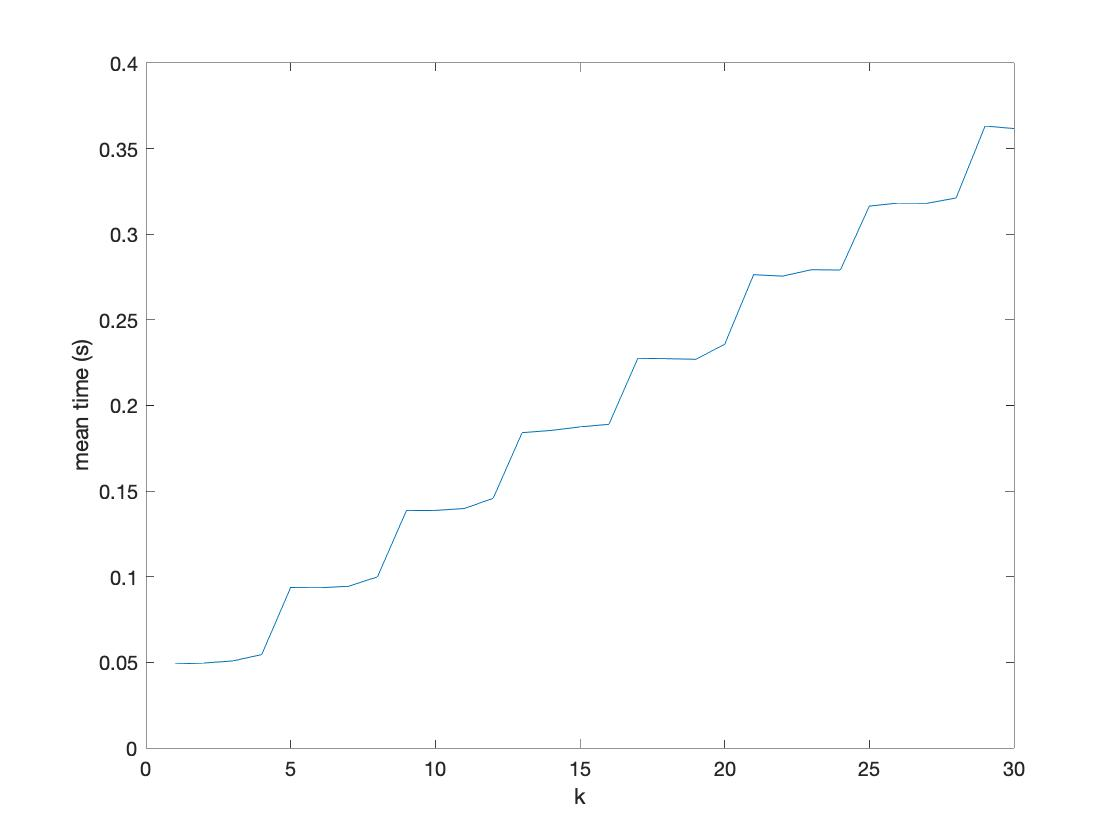
\includegraphics[width=0.8\columnwidth]{Figures/Task4tvk_parrallel.jpg}
        \caption{\label{fig:Task4_1b}After parralleisation
        }
    \end{subfigure}
    \caption{The mean time in seconds for the calculation of the refined neural network outputs across all examples from Task 4 against $k$  . With $k_{max}=30$ before and after parralleisation}
    \label{fig:Task4_1}
\end{figure}
\subsubsection{Discussion}
% Projected gradient ascent allows us to obtain a better lower bound on $y_{max}$ than interval bound propogation. 
% However, it does not achieve a lower bound as high as random sampling while being significantly more computationally expensive. 
% This is possibly because of the limitation on the domain
\texttt{projected\_gradient\_ascent} does not provide sufficiently improved bounds over \texttt{random\_sampling} to justify the multiple order of magnitude increase in computation time required.
In the \texttt{branch\_and\_bound} procedure we see many fewer convergences as the time per iteration is increased and thus fewer iterations are completed within the time limit.
% The reason we see a drop in computation time by a factor of four upon parralleisation is that that is the number of cores in our machine and thus the number of processes we were able to run in parallel.
The main problem with the procedure comes from keeping $\boldsymbol{x}^{refined}$ within the domain.
A possible improvement to this procedure would be the use of techniques to adjust the learning rate as the procedure runs for example learning rate decay or momentum.
Our choices of hyperparameters in this task reflects the need to balance the quality of the bounds and the computation time.

%----------------------------------------------------------------------------------------
%	TASK 5
%----------------------------------------------------------------------------------------

\subsection{Task 5 - Linear Programming Bound}
\subsubsection{Method}
\paragraph{Function \texttt{interval\_bound\_propogation\_comprehensive}}
This function works much like the function from Task 2 \texttt{interval\_bound\_propogation}. However, it records and returns the bounds on every layer of the network.

\paragraph{Function \texttt{calculate\_num\_constraints}} This calculates the number of equalities and inequalities that will be generated by the program in order to be able to allocate the correct amount of memory for the matracies.

\paragraph{Function \texttt{generate\_constraints}} 
This creates the $\boldsymbol{A}$, $\boldsymbol{A}_{eq}$, $\boldsymbol{b}$ and $\boldsymbol{b}_{eq}$ matracies coding for the given constraints.
It is notable that the number of equalities and inequalities varies with the bounds on each neuron due to the nature of the ReLU. 
If $z^{max}_{l_i}<0$ then we are able to set $z_{l_i}=0$ and if $z^{min}_{l_i}>0$ then we are able to set $z_{l_i}=\hat{z}_{l_i}$. 
Otherwise we need to use three inequalities to bound the ReLU as explained in~\cite{NNVNotes}.

\paragraph{Function \texttt{linear\_programming\_bound}} This generates an upper and lower bound on $y$ using the \texttt{matlab} function \texttt{linprog}. 
First we generate bounds using \texttt{interval\_bound\_propogation\_comprehensive} and pass that, along with the result from \texttt{calculate\_num\_constraints}, into \texttt{generate\_constraints}.
We then define our cost function to be minimised, which is simply $\hat{z}_5$ for the lower bound and $-\hat{z}_5$ for the upper bound. 
We finally run \texttt{linprog} with each of these two cost functions to obtain $y_{lb}$ and $y_{ub}$.

\paragraph{Script} This works much like \textbf{Algorithm \ref{alg:Task2}} however we use \texttt{linear\_programming\_bound} in the place of \texttt{interval\_bound\_propogation}.

\paragraph{Branch and Bound} We ran the \texttt{branch\_and\_bound} procedure using a version of \texttt{linear\_programming\_bound} which only generated upper bounds to save on computation time. We generated lower bounds with \texttt{random\_sampling}.
\subsubsection{Results}
The plots for Task 5 are show in figure \ref{fig:Task5}. 
We obtained a mean lower bound on $y$ of -77.6 and a mean upper bound on $y$ of 14.8. 
We were also able to correctly classify 0 examples as false and 126 examples as true. 
When used in the \texttt{branch\_and\_bound} procedure with $\epsilon=0.025$ and $k=500$ for \texttt{random\_sampling} we were able to correctly classify all 500 properties. 
The computation time was significantly shorter than when using \texttt{interval\_bound\_propogation} to genereate upper bounds.
% \begin{figure}
%     \centering

%         \centering 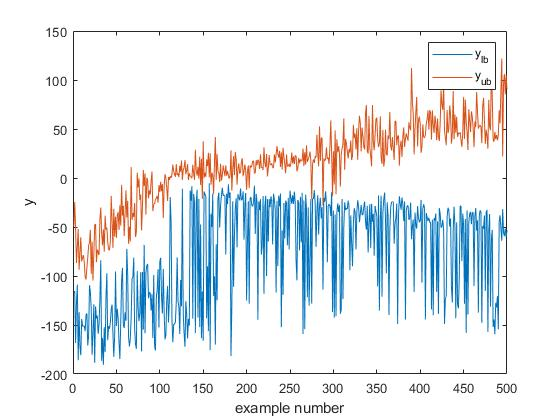
\includegraphics[scale=0.4]{Figures/Task5.jpg}
%     \caption{The upper and lower bounds on $y$ as obtained by linear programming bound in Task 5 against example number}
%     \label{fig:Task5}
% \end{figure}
\begin{figure}
    \centering
    \begin{subfigure}{.5\textwidth} 
        \centering 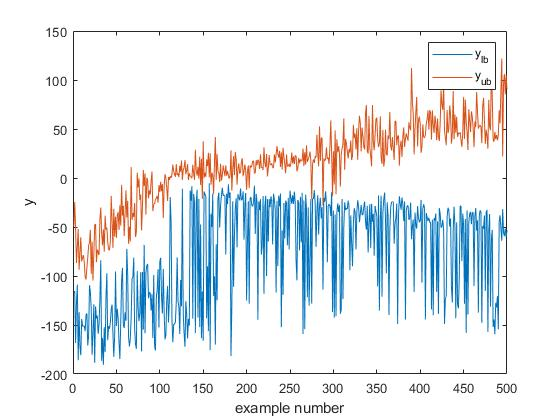
\includegraphics[width=0.8\columnwidth]{Figures/Task5.jpg}
        \caption{The upper and lower bounds on $y$ as obtained by \texttt{linear\_programming\_bound} in Task 5 against example number}
        \label{fig:Task5a}
    \end{subfigure}%
    \begin{subfigure}{.5\textwidth} 
        \centering 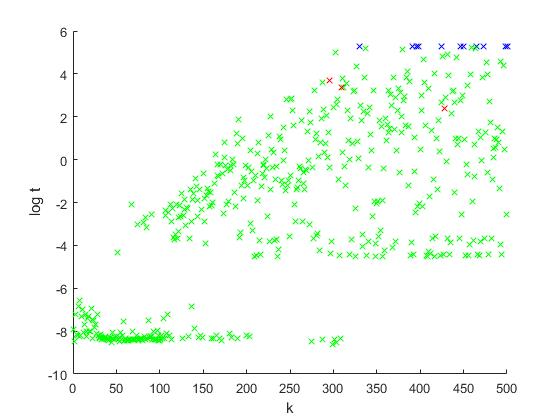
\includegraphics[width=0.8\columnwidth]{Figures/Task5bandb.jpg}
        \caption{The log of the time taken for the \texttt{branch\_and\_bound} procedure to converge in Task 5 against the example number. Examples classified correctly are shown in green and examples which did not converge are shown in blue.}
        \label{fig:Task5b}
    \end{subfigure}
    \caption{The bounds generated by \texttt{linear\_programming\_bound} in Task 5 and the results when this is used in the \texttt{branch\_and\_bound} procedure.}
    \label{fig:Task5}
\end{figure}
\subsubsection{Discussion}
The \texttt{linear\_programming\_bound} method produces much tighter bounds than \texttt{interval\_bound\_propogation}. 
The upper bounds are significantly decreased from the previous best, however, compared to \texttt{random\_sampling} and \texttt{projected\_gradient\_ascent} the lower bounds are very loose. 
This is because this method finds bounds on $y$ rather than $y^*$ much like \texttt{interval\_bound\_propogation}.
We chose to only optimize the bounds of the output node in this task as it significantly reduced potential computation time. 
A way we could improve the bounds is to perform the optimisation on every node in the network from input to output. 
This would result in very tight bounds. 
When used with the \texttt{branch\_and\_bound} method we found some false examples were falsely classified with $\epsilon \geq 0.3$ due to their $y^*$ being less than this. Once we lowered $\epsilon$ to $0.25$ all examples were correctly classified.

\section{Conclusion}

We have discussed and evaluated our approaches to Neural Network Verification methods. 
% A common theme we have discussed is the difference between finding bounds on $y$ and $y_{max}$ and how this affects the \texttt{branch\_and\_bound} procedure.
We were able to correctly classify all 500 examples from the collision detection dataset through choosing the most computationally effective methods and adjusting hyperparameters. 
Our work has only explored methods of bounding $y$ and $y^*$ which were utilised in the \texttt{branch\_and\_bound} procedure to classify examples.
% Further work could explore the effectiveness of these methods on other, harder datasets or explore new methods entirely. 
Further work could explore different methods of bounding such as the extended \texttt{linear\_programming\_bound} method discussed in Task 5.
Other areas for further work could include looking into other methods for picking out and splitting domains in the \texttt{branch\_and\_bound} procedure.

%----------------------------------------------------------------------------------------
%	BIBLIOGRAPHY
%----------------------------------------------------------------------------------------
% \scriptsize {
\setstretch{1.3}
\bibliographystyle{plain}

\bibliography{sample}
% }
%----------------------------------------------------------------------------------------

\end{document}